\documentclass{article}
\usepackage{microtype}
\usepackage{graphicx}
\usepackage{booktabs,array}
\usepackage{xcolor}
\usepackage{hyperref,xurl}
\usepackage{placeins}
% The supplied ICML style is unchanged. This is a working preprint.
\usepackage[preprint]{icml2027}
\usepackage{amsmath,amssymb,mathtools,amsthm}
\usepackage[capitalize,noabbrev]{cleveref}
\usepackage{enumitem}
\usepackage{listings}
\newtheorem{proposition}{Proposition}
\newcommand{\U}{\mathbf U}
\newcommand{\D}{\mathbf D}
\newcommand{\pending}{\textit{Pending}}
\newcommand{\valOrderMin}{1.999}
\newcommand{\valOrderMax}{2.001}
\newcommand{\expoRatio}{4.00}
\newcommand{\expoMax}{\ensuremath{2.4\times10^{-4}}}
\newcommand{\pilotSpearmanMin}{0.99998}
\newcommand{\pilotFlips}{2}
\newcommand{\pilotTriplets}{7,344}
\newcommand{\pilotMaxU}{0.773}
\newcommand{\pilotMaxV}{0.734}
\newcommand{\simSeconds}{40}
\newcommand{\simOOR}{637}
\newcommand{\simMin}{\ensuremath{-2.9\times10^{-16}}}
\newcommand{\simMax}{0.753}
\newcommand{\refEpsLinear}{\ensuremath{2.3\times10^{-9}}}
\newcommand{\refEpsNonlinear}{\ensuremath{3.3\times10^{-9}}}
\newcommand{\refResolvedMin}{100.0}
\newcommand{\refCertified}{10.3}
\newcommand{\refUnresolved}{0}
\newcommand{\refDFiveHundred}{0.959}
\newcommand{\refSubsetVsAll}{0.997}
\newcommand{\refDmin}{\ensuremath{2.6\times10^{-5}}}
\newcommand{\refDmax}{0.086}
\newcommand{\spGemText}{0.21}
\newcommand{\trGemText}{0.57}
\newcommand{\spGemImage}{0.76}
\newcommand{\trGemImage}{0.78}
\newcommand{\spGemBoth}{0.23}
\newcommand{\trGemBoth}{0.58}
\newcommand{\spQwText}{0.44}
\newcommand{\trQwText}{0.65}
\newcommand{\spQwImage}{0.78}
\newcommand{\trQwImage}{0.79}
\newcommand{\spQwBoth}{0.39}
\newcommand{\trQwBoth}{0.66}
\newcommand{\spGmeText}{0.46}
\newcommand{\trGmeText}{0.64}
\newcommand{\spGmeImage}{0.83}
\newcommand{\trGmeImage}{0.84}
\newcommand{\spGmeBoth}{0.50}
\newcommand{\trGmeBoth}{0.67}
\newcommand{\spGemTextSame}{$-$0.26}
\newcommand{\spGemTextCh}{0.32}
\newcommand{\spGemTextHund}{0.24}
\newcommand{\spGemTextFull}{0.28}
\newcommand{\spGemTextPhys}{0.30}
\newcommand{\trGemTextCert}{0.70}
\newcommand{\ciGemText}{[0.21, 0.23]}
\newcommand{\rangeLoGemText}{0.9846}
\newcommand{\rangeHiGemText}{0.9989}
\newcommand{\facGemText}{0.997/0.992/0.990}
\newcommand{\spGemImageSame}{0.64}
\newcommand{\spGemImageCh}{0.80}
\newcommand{\spGemImageHund}{0.70}
\newcommand{\spGemImageFull}{0.83}
\newcommand{\spGemImagePhys}{0.62}
\newcommand{\trGemImageCert}{0.79}
\newcommand{\ciGemImage}{[0.73, 0.79]}
\newcommand{\rangeLoGemImage}{0.9968}
\newcommand{\rangeHiGemImage}{1.0000}
\newcommand{\facGemImage}{1.000/0.999/0.999}
\newcommand{\spGemBothSame}{$-$0.09}
\newcommand{\spGemBothCh}{0.33}
\newcommand{\spGemBothHund}{0.25}
\newcommand{\spGemBothFull}{0.39}
\newcommand{\spGemBothPhys}{0.29}
\newcommand{\trGemBothCert}{0.70}
\newcommand{\ciGemBoth}{[0.22, 0.24]}
\newcommand{\rangeLoGemBoth}{0.9803}
\newcommand{\rangeHiGemBoth}{0.9990}
\newcommand{\facGemBoth}{0.996/0.993/0.990}
\newcommand{\revOrigGem}{0.75}
\newcommand{\revRevGem}{0.81}
\newcommand{\revSelfGem}{0.9989}
\newcommand{\revCorrGem}{0.95}
\newcommand{\notTopGem}{0.38}
\newcommand{\notSelfGem}{0.973}
\newcommand{\notOtherGem}{0.998}
\newcommand{\notSpGem}{0.21}
\newcommand{\notCloserGem}{53}
\newcommand{\notAllGem}{83\%}
\newcommand{\notSpOrigGem}{0.21}
\newcommand{\misImgGem}{0.41}
\newcommand{\misDeckGem}{0.19}
\newcommand{\misBothGem}{0.22}
\newcommand{\heatGem}{preserved}
\newcommand{\heatValsGem}{0.9991/0.9978/0.9969}
\newcommand{\ffDiffGem}{0}
\newcommand{\spQwTextSame}{0.22}
\newcommand{\spQwTextCh}{0.53}
\newcommand{\spQwTextHund}{0.36}
\newcommand{\spQwTextFull}{0.20}
\newcommand{\spQwTextPhys}{0.23}
\newcommand{\trQwTextCert}{0.66}
\newcommand{\ciQwText}{[0.39, 0.45]}
\newcommand{\rangeLoQwText}{0.8984}
\newcommand{\rangeHiQwText}{0.9963}
\newcommand{\facQwText}{0.991/0.951/0.943}
\newcommand{\spQwImageSame}{0.69}
\newcommand{\spQwImageCh}{0.82}
\newcommand{\spQwImageHund}{0.88}
\newcommand{\spQwImageFull}{0.77}
\newcommand{\spQwImagePhys}{0.94}
\newcommand{\trQwImageCert}{0.83}
\newcommand{\ciQwImage}{[0.73, 0.83]}
\newcommand{\rangeLoQwImage}{0.9872}
\newcommand{\rangeHiQwImage}{0.9991}
\newcommand{\facQwImage}{0.998/0.992/0.992}
\newcommand{\spQwBothSame}{0.11}
\newcommand{\spQwBothCh}{0.49}
\newcommand{\spQwBothHund}{0.34}
\newcommand{\spQwBothFull}{0.22}
\newcommand{\spQwBothPhys}{0.29}
\newcommand{\trQwBothCert}{0.65}
\newcommand{\ciQwBoth}{[0.35, 0.40]}
\newcommand{\rangeLoQwBoth}{0.8816}
\newcommand{\rangeHiQwBoth}{0.9972}
\newcommand{\facQwBoth}{0.992/0.941/0.937}
\newcommand{\revOrigQw}{0.70}
\newcommand{\revRevQw}{0.74}
\newcommand{\revSelfQw}{0.9875}
\newcommand{\revCorrQw}{0.84}
\newcommand{\notTopQw}{0.77}
\newcommand{\notSelfQw}{0.956}
\newcommand{\notOtherQw}{0.995}
\newcommand{\notSpQw}{0.35}
\newcommand{\notCloserQw}{15}
\newcommand{\notAllQw}{0\%}
\newcommand{\notSpOrigQw}{0.45}
\newcommand{\misImgQw}{0.09}
\newcommand{\misDeckQw}{0.36}
\newcommand{\misBothQw}{0.37}
\newcommand{\heatQw}{preserved}
\newcommand{\heatValsQw}{0.9963/0.9912/0.9896}
\newcommand{\ffDiffQw}{0}
\newcommand{\spGmeTextSame}{0.18}
\newcommand{\spGmeTextCh}{0.55}
\newcommand{\spGmeTextHund}{0.49}
\newcommand{\spGmeTextFull}{0.29}
\newcommand{\spGmeTextPhys}{0.57}
\newcommand{\trGmeTextCert}{0.69}
\newcommand{\ciGmeText}{[0.44, 0.47]}
\newcommand{\rangeLoGmeText}{0.9727}
\newcommand{\rangeHiGmeText}{0.9983}
\newcommand{\facGmeText}{0.997/0.984/0.981}
\newcommand{\spGmeImageSame}{0.74}
\newcommand{\spGmeImageCh}{0.86}
\newcommand{\spGmeImageHund}{0.87}
\newcommand{\spGmeImageFull}{0.74}
\newcommand{\spGmeImagePhys}{0.89}
\newcommand{\trGmeImageCert}{0.87}
\newcommand{\ciGmeImage}{[0.75, 0.84]}
\newcommand{\rangeLoGmeImage}{0.9853}
\newcommand{\rangeHiGmeImage}{0.9988}
\newcommand{\facGmeImage}{0.997/0.990/0.990}
\newcommand{\spGmeBothSame}{0.26}
\newcommand{\spGmeBothCh}{0.59}
\newcommand{\spGmeBothHund}{0.54}
\newcommand{\spGmeBothFull}{0.53}
\newcommand{\spGmeBothPhys}{0.58}
\newcommand{\trGmeBothCert}{0.76}
\newcommand{\ciGmeBoth}{[0.47, 0.54]}
\newcommand{\rangeLoGmeBoth}{0.9722}
\newcommand{\rangeHiGmeBoth}{0.9977}
\newcommand{\facGmeBoth}{0.995/0.983/0.980}
\newcommand{\revOrigGme}{0.77}
\newcommand{\revRevGme}{0.74}
\newcommand{\revSelfGme}{0.9849}
\newcommand{\revCorrGme}{0.68}
\newcommand{\notTopGme}{0.50}
\newcommand{\notSelfGme}{0.958}
\newcommand{\notOtherGme}{0.997}
\newcommand{\notSpGme}{0.42}
\newcommand{\notCloserGme}{53}
\newcommand{\notAllGme}{93\%}
\newcommand{\notSpOrigGme}{0.44}
\newcommand{\misImgGme}{0.41}
\newcommand{\misDeckGme}{0.40}
\newcommand{\misBothGme}{0.46}
\newcommand{\heatGme}{not preserved}
\newcommand{\heatValsGme}{0.9987/0.9990/0.9991}
\newcommand{\ffDiffGme}{0}
\newcommand{\spTextMin}{0.21}
\newcommand{\spTextMax}{0.46}
\newcommand{\trTextMin}{0.57}
\newcommand{\trTextMax}{0.65}
\newcommand{\spImageMin}{0.76}
\newcommand{\spImageMax}{0.83}
\newcommand{\trImageMin}{0.78}
\newcommand{\trImageMax}{0.84}
\newcommand{\spBothMin}{0.23}
\newcommand{\spBothMax}{0.50}
\newcommand{\trBothMin}{0.58}
\newcommand{\trBothMax}{0.67}
\newcommand{\spTfidf}{0.35}
\newcommand{\trTfidf}{0.61}
\newcommand{\spTfidfSame}{0.26}
\newcommand{\spTfidfFull}{0.67}
\newcommand{\spTfidfAll}{0.36}
\newcommand{\spPix}{0.93}
\newcommand{\trPix}{0.95}
\newcommand{\spPixSame}{0.90}
\newcommand{\spPixFull}{0.99}
\newcommand{\spPixAll}{0.95}
\newcommand{\spFour}{0.44}
\newcommand{\trFour}{0.73}
\newcommand{\spFourSame}{0.20}
\newcommand{\spFourFull}{0.40}
\newcommand{\spFourAll}{0.42}
\newcommand{\spPhys}{0.82}
\newcommand{\trPhys}{0.90}
\newcommand{\spPhysSame}{0.74}
\newcommand{\spPhysFull}{0.64}
\newcommand{\spPhysAll}{0.83}
\newcommand{\failGem}{0}
\newcommand{\failQw}{0}
\newcommand{\failGme}{0}
\newcommand{\precTextMinCos}{0.99995}
\newcommand{\precTextSS}{0.999}
\newcommand{\precTextRefA}{0.22}
\newcommand{\precTextRefB}{0.22}
\newcommand{\precImageMinCos}{0.99996}
\newcommand{\precImageSS}{0.990}
\newcommand{\precImageRefA}{0.72}
\newcommand{\precImageRefB}{0.70}
\newcommand{\precBothMinCos}{0.99990}
\newcommand{\precBothSS}{0.997}
\newcommand{\precBothRefA}{0.21}
\newcommand{\precBothRefB}{0.22}

\renewcommand{\today}{November 19, 2026}
\icmltitlerunning{Do Multimodal Embeddings Capture PDE Behavior?}
\hypersetup{pdftitle={Do Multimodal Embeddings Capture PDE Behavior?},pdfauthor={Anonymous Authors},pdfsubject={Working research manuscript}}
\begin{document}
\twocolumn[
\icmltitle{Do Multimodal Embeddings Capture PDE Behavior?}
\begin{icmlauthorlist}
\icmlauthor{Anonymous Authors}{anon}
\end{icmlauthorlist}
\icmlaffiliation{anon}{Affiliations omitted in this working draft}
\icmlcorrespondingauthor{Anonymous Authors}{contact omitted in this draft}
\icmlkeywords{PDEs, multimodal embeddings, representation evaluation, scientific machine learning}
\vskip 0.3in
]
\printAffiliationsAndNotice{}
\begin{abstract}
Can a pretrained embedding model tell when two partial differential equation (PDE) problems lead to similar behavior? We test this on 54 two-dimensional problems built from six equations, three kinds of initial condition, and three boundary conditions, each simulated 100 times with one validated solver. The similarity of two problems is the root-mean-square difference between their solutions when both start from the same initial data, and numerical error bounds show that every ranking we use is reliable. We then give three multimodal embedding models, used without fine-tuning, a text description of each problem, an image of five snapshots of its solution, or both. We ask whether their similarity scores rank pairs of problems in the same order. On ten samples per problem, chosen in advance, image embeddings reach Spearman correlations of \spImageMin--\spImageMax{} with the reference, while simply comparing pixels reaches \spPix{}. Text embeddings reach only \spTextMin--\spTextMax{}, close to a character $n$-gram baseline (\spTfidf{}). For two of the models, rewriting a description in equivalent notation moves its embedding further than replacing the problem with any of the other 53. Text and image together give \spBothMin--\spBothMax{}, close to text alone. These models recognize solutions that look alike much better than equations that behave alike.
\end{abstract}
\noindent\textbf{Draft status.} All simulations, reference distances, and simple baselines are complete. Because only CPU hardware was available, the embedding models were run on 10 of the 100 samples per problem, chosen in advance. The full run is still to be done.
\section{Introduction}
Two PDEs can look almost the same on paper and still produce very different solutions. The reverse is also common: one problem can be written in many equivalent ways. A representation that helps scientists find related problems should cope with both situations. It should place problems with similar solutions close together, and it should not be thrown off by a change of notation.

General-purpose embedding models are already used to search and organize scientific text and images, and many of them accept text, images, or both. It is natural to ask whether their similarity scores say anything about how PDE solutions behave. We ask a narrow version of this question: \emph{when an embedding model rates one pair of problems as more similar than another, do the solutions of the first pair actually evolve more similarly?} A positive answer on our benchmark would not show general mathematical reasoning. A negative answer would show that these embedding spaces should not be read as statements about dynamics.

Answering the question requires a ground truth, which we build by simulation. We take six equations with two fields on the unit square, three families of initial conditions (ICs), and three boundary conditions (BCs). We call each combination of equation, IC family, and BC a \emph{problem}. For each of the 54 problems we simulate 100 samples, giving 5,400 trajectories. Problems in the same IC family start from exactly the same initial fields. This lets us compare them directly: start two systems from the same state and measure how far apart their solutions drift. Our reference distance is the root-mean-square (RMS) difference between the fields.

We then query three multimodal embedding models, used as released and without fine-tuning, in three ways: with a text description of the problem, with an image of five solution snapshots, and with both together. In each case we compare the models' similarity rankings with the reference rankings. Simple baselines and a set of controls help interpret the results.

The answer is mostly negative. Images give moderate agreement with the reference, but comparing the raw pixels gives more. Text descriptions give weak agreement, about the same as matching character sequences. They are also fragile: for two of the models, writing the same problem in different notation changes the embedding more than switching to any other problem in the benchmark. Giving the model the image together with the text helps little.

Our contributions are:
\begin{itemize}[leftmargin=*,itemsep=1pt,topsep=2pt]
\item a benchmark of 5,400 simulated trajectories, produced by one validated solver, each with a complete text description that never names the equation;
\item a reference distance with numerical error bounds, which show that every ranking we use is reliable, and prove it exactly for the linear equations;
\item an evaluation of three embedding models with text, image, and joint inputs, together with baselines and controls. Because only CPU hardware was available, the models were evaluated on 10 of the 100 samples per problem, chosen in advance.
\end{itemize}
The mathematical tools are classical: Euclidean distance, matrix exponentials, and standard time stepping. What is new is the controlled evidence.

\paragraph{Related work.}
APEBench provides configurable PDE benchmarks and reference solvers \citep{koehler2024apebench}. Physics-informed contrastive learning trains PDE representations with physical information \citep{lorsung2024picl}, and Unisolver and PDEformer condition learned solvers on the equation \citep{zhou2025unisolver,ye2024pdeformer}. We instead keep general-purpose encoders fixed and study the geometry they already have. Work on mathematical equivalence in embedding models, such as MELD, motivates our notation controls \citep{ye2026meld}. We extend that question from formulas to descriptions and images of evolving fields, where the ICs, BCs, and observation times all matter.

\section{The Benchmark}
\label{sec:benchmark}
\subsection{Six Equations}
All six equations act on the same pair of dimensionless fields, $\U=(u,v)^\top$, on the unit square $\Omega=[0,1]^2$. Each has diffusion plus one extra term:
\begin{equation}
 \partial_t\U=\D\Delta\U+G(\U,\nabla\U),
 \qquad \D=\operatorname{diag}(\nu_u,\nu_v).
\label{eq:common-pde}
\end{equation}
\Cref{tab:equations} lists the six choices of $G$. In four equations the two fields evolve independently; in linear exchange and Gray--Scott they interact. Because every equation uses the same two fields, any two problems can be compared directly, without padding missing fields or matching unrelated physical quantities.

\begin{table*}[t]
\centering
\caption{The six equations. All have the form $\partial_t\U=\D\Delta\U+G$ on the same square. Products and powers act pointwise. They are six small parabolic models, not a survey of PDE types.}
\label{tab:equations}
\small
\begin{tabular}{p{0.22\textwidth}p{0.48\textwidth}p{0.22\textwidth}}
\toprule
Equation & Extra term $G$ & Behavior \\
\midrule
Diffusion & $(0,0)^\top$ & Smoothing; linear reference \\
Advection--diffusion & $-c_x\partial_x\U-c_y\partial_y\U$ & Transport and smoothing \\
Linear exchange & $\kappa(v-u,\ u-v)^\top$ & Coupling; linear reference \\
Fisher--KPP & $r\big(u(1-u),\ v(1-v)\big)^\top$ & Logistic growth \\
Allen--Cahn (shifted) & $a\big(u(1-u)(u-\tfrac12),\ v(1-v)(v-\tfrac12)\big)^\top$ & Two stable states \\
Gray--Scott & $\big(-uv^2+F(1-u),\ uv^2-(F+k)v\big)^\top$ & Nonlinear coupling \\
\bottomrule
\end{tabular}
\end{table*}

We use one coefficient setting per equation: $\nu_u=0.01$, $\nu_v=0.005$, $c=(0.25,0.10)$, $\kappa=0.5$, $r=1$, $a=4$, $F=0.04$, and $k=0.06$. Before the main run, a small pilot on samples that are not part of the test set (indices 100--119) checked these values against criteria written down beforehand (\cref{app:pilot}). Every solution changes visibly: the smallest average relative change from $t=0$ to $t=1$ is 0.37. Every equation separates from pure diffusion by much more than the time-stepping error (at least $5.3\times10^{-3}$ in RMS, against about $2\times10^{-10}$). The Allen--Cahn initial fields fall on both sides of its threshold $\tfrac12$ (19 of 120 pilot fields peak above it). All checks passed, so the coefficients were kept. No embedding model was used in the pilot. With one setting per equation, the results say nothing about an entire PDE family.

\subsection{Initial and Boundary Conditions}
The three IC families are a single smooth bump, low-frequency oscillations, and a mix of three smooth patches. Each field draws its own random parameters. Every IC is multiplied by the same smooth window
\begin{equation}
 w(x,y)=\eta(x)\eta(y),\qquad
 \eta(s)=\exp\!\left(4-\frac{1}{s(1-s)}\right)
\label{eq:window}
\end{equation}
for $0<s<1$, with $\eta(0)=\eta(1)=0$. The window makes the initial values and all their derivatives vanish at the boundary. The same initial field is therefore valid for all three BCs, and changing the BC never changes the starting pattern. (This covers the initial data only; we assume no extra compatibility at the corners.)

The BCs are periodic in both directions, zero Dirichlet ($\U=0$ on $\partial\Omega$), and zero Neumann ($\partial_n\U=0$). For advection--diffusion, the Neumann condition sets the normal gradient to zero, not the total flux. Every equation keeps some diffusion, so pure transport, which would need different boundary data, never appears.

Within an IC family, the same 100 initial arrays are used for all six equations and all three BCs. Different families are linked through a shared random seed, so comparisons across families also include the change in initial data. Initial values lie in $[0,0.8]$. We do not assume that solutions stay in this range, and no field is ever clipped.

\subsection{Simulation}
\label{sec:simulator}
The benchmark has $6\times3\times3=54$ problems and 5,400 trajectories. Each trajectory stores 100 states, including the initial one, at times $t_n=n/99$ for $n=0,\ldots,99$, so the time horizon is $T=1$. The full float32 array has shape $[54,\ 100,\ 100,\ 2,\ 64,\ 64]$ (problem, sample, time, field, and the two space directions) and takes about 17.7\,GB.

APEBench and its Exponax solvers use Fourier methods on periodic domains \citep{koehler2024apebench,apebench_docs,exponax_docs}. Because we also need Dirichlet and Neumann BCs, we wrote one small finite-difference solver for all 54 problems. It uses the five-point Laplacian on a $64\times64$ cell-centered grid, with ghost values that wrap around (periodic), flip sign (Dirichlet), or copy the neighbor (Neumann). For each BC this matrix is diagonalized exactly by a fast transform: the real FFT, the DST-II, or the DCT-II. Diffusion is therefore solved exactly in that basis. Advection uses centered differences with the same ghost values; the exchange and reaction terms act pointwise. Time stepping uses ETDRK4 \citep{cox2002etd,kassam2005etdrk4} with four steps per output interval ($\delta t=1/396$), computed in float64 and stored in float32.

We tested the solver before the main run (\cref{app:validation}). For the three linear equations, its output matches the exact solution of the same grid equations to within $2.3\times10^{-10}$. For the nonlinear equations, using four times as many steps changes no value by more than $5\times10^{-12}$, and the error shrinks at the expected fourth-order rate. In space the solver converges at second order for every BC, and the five-frame RMS difference between the $64\times64$ and $256\times256$ grids is at most $4.0\times10^{-4}$ (median $8\times10^{-5}$). An independent periodic solver, Exponax, gives the same picture. Our reference is the solution on the $64\times64$ grid; the finer grids only show how close that solution is to the continuous PDE.

\subsection{Text Descriptions}
Each sample of each problem has a plain-text description written in LaTeX. It gives the two equations with their coefficients, the explicit initial fields with their sampled parameters, the BC, the domain, and the observation times. A random seed alone would not tell a model what the initial field is, so the description states the actual formula. Headings are generic, such as ``Equation'' and ``Boundary''. The description never names the equation, the problem, or the solver; this information is kept in a separate record. A generator script produces all 5,400 descriptions.

\section{Measuring Similarity}
\label{sec:comparison}
\subsection{A Distance Between Problems}
The image models see five snapshots of each solution, at time indices
\[
 \mathcal I=\{0,25,50,74,99\},\qquad Q=5.
\]
We compare problems on these same snapshots. Let $X_i^{(r)}\in\mathbb R^{Q\times C\times H\times W}$ hold the five snapshots of sample $r$ of problem $i$, with $C=2$ fields, $H=W=64$, and $N=100$ samples. The reference distance is
\begin{equation}
 \boxed{D_{ij}=\left[
 \frac{1}{NQCHW}\sum_{r=1}^{N}
 \left\|X_i^{(r)}-X_j^{(r)}\right\|_F^2
 \right]^{1/2}.}
\label{eq:rms}
\end{equation}
This is the RMS difference between the two solutions, averaged over samples that share their initial data. A small value means that the two problems evolve similarly for these ICs, this time horizon, and these field scales. We also report a version that uses all 100 saved states. Five snapshots give a discrete average; we do not claim that they represent the full continuous-time behavior.

\begin{proposition}[Distance on observed behavior]
Stack the scaled snapshots of problem $i$ into one vector $F_i$. Then $D_{ij}=\|F_i-F_j\|_2$, so $D$ is symmetric, nonnegative, and satisfies the triangle inequality. It is a metric on distinct recorded solutions and a pseudometric on problems.
\label{prop:distance}
\end{proposition}
The second statement is a reminder that two equations could agree on these samples and times but differ elsewhere. The proof and the exact scaling are in \cref{app:trajectory-distance}.

\paragraph{Which pairs we compare.}
Our main comparisons hold the IC family fixed. Each family gives an $18\times18$ matrix covering the six equations and three BCs, all started from the same initial arrays. The full $54\times54$ matrix also compares problems from different IC families, so it mixes the effect of the equation with the effect of the initial data. We treat it as a secondary result.

\subsection{From Distances to Dot Products}
Embedding models report similarity as a dot product, so it helps to write the reference the same way. With the kernel $K_{ij}=F_i^\top F_j$,
\begin{equation}
 D_{ij}^2=K_{ii}+K_{jj}-2K_{ij}.
\label{eq:raw-kernel}
\end{equation}
This links the distance to an inner product while keeping the size of each field.

For an embedding model, let $z_i^{(r)}$ be the unit-length embedding of sample $r$ of problem $i$. We average the dot products over samples:
\begin{equation}
 S_{ij}^{\mathrm{emb}}=
 \frac1N\sum_{r=1}^{N}z_i^{(r)\top}z_j^{(r)}.
\label{eq:embedding-score}
\end{equation}
The matching embedding distance satisfies
\begin{equation}
 (d_{ij}^{\mathrm{emb}})^2
 =\frac1N\sum_r\|z_i^{(r)}-z_j^{(r)}\|_2^2
 =2-2S_{ij}^{\mathrm{emb}},
\label{eq:chord}
\end{equation}
so a larger dot product always means a smaller distance. We only ask whether $S^{\mathrm{emb}}$ ranks pairs in the same order as $-D$; the actual values need not match.

We also use a \emph{physical cosine}: normalize each simulated solution to unit length and then average the paired dot products, exactly as in \cref{eq:embedding-score}. This score ignores how large a response is and keeps only its shape. It can rank pairs differently from $D$, so we report it separately (\cref{app:physical-kernel}).

\subsection{Calibration With Exact Solutions}
For diffusion and linear exchange, each Laplacian mode evolves independently:
\begin{equation}
 \widehat\U_\ell(t)
 =\exp\!\big[t(\lambda_\ell\D+R)\big]
 \widehat\U_\ell(0),
\label{eq:linear-reference}
\end{equation}
with $R=0$ or $R=\kappa\left(\begin{smallmatrix}-1&1\\1&-1\end{smallmatrix}\right)$ \citep{higham2008functions}. The eigenvalues and eigenvectors of our grid Laplacian are known for each BC, so this formula gives the grid solution with no time-stepping error, apart from rounding. Advection--diffusion can be solved exactly in a similar way (\cref{app:linear-reference}).

A continuous example makes the scale of $D$ concrete. For the heat equation with zero Dirichlet BC and $u_0=\sin(\pi x)\sin(\pi y)$, the solution is $u_\nu(t,x,y)=e^{-2\pi^2\nu t}\sin(\pi x)\sin(\pi y)$. Over the five observed times, the RMS difference between two diffusion coefficients is
\begin{equation}
 D(\nu,\nu')=\frac12
 \left[\frac15\sum_{n\in\mathcal I}
 \big(e^{-2\pi^2\nu t_n}-e^{-2\pi^2\nu't_n}\big)^2
 \right]^{1/2}.
\label{eq:heat-example}
\end{equation}
\Cref{tab:calibration} gives values from this formula. They are exact calculations, not simulations or embedding results, and this IC is not one of the benchmark families. We later use the same four coefficients to test whether text embeddings notice a change of a single number.

\begin{table}[t]
\centering
\caption{Exact heat-equation distances from \cref{eq:heat-example}, relative to $\nu=0.01$. An embedding that tracks behavior should rank the candidates in this order.}
\label{tab:calibration}
\begin{tabular}{ccc}
\toprule
Candidate $\nu'$ & Five-frame RMS & 100-frame RMS \\
\midrule
0.011 & 0.005100 & 0.004895 \\
0.020 & 0.047511 & 0.045899 \\
0.050 & 0.152800 & 0.150418 \\
\bottomrule
\end{tabular}
\end{table}

\subsection{When Can We Trust a Ranking?}
Simulated distances contain numerical error, and a small error could swap two nearly equal distances. The following bound says when that cannot happen.
\begin{proposition}[A sufficient numerical margin]
Suppose $\|F_i-\widetilde F_i\|_2\le\epsilon_i$, where $\widetilde F_i$ is the computed solution. Then
\begin{equation}
 |D_{ij}-\widetilde D_{ij}|\le\epsilon_i+\epsilon_j.
\end{equation}
If $\widetilde D_{ik}-\widetilde D_{ij}>2\epsilon_i+\epsilon_j+\epsilon_k$, then the exact distances satisfy $D_{ij}<D_{ik}$.
\label{prop:margin}
\end{proposition}
The proof is the reverse triangle inequality. The bound is only as good as the error estimates $\epsilon_i$. For the linear equations we compute $\epsilon_i$ against exact solutions, so a ranking that passes the test is proved, up to rounding. For the nonlinear equations we estimate $\epsilon_i$ by refining the time step; this is strong evidence but not a proof.

\section{Experimental Setup}
\label{sec:experiment}
\subsection{Models and Inputs}
We test the three models in \cref{tab:model-inputs}. Each one accepts text, images, and text and image together \citep{embeddinggemma2_modelcard,qwen3vl_embedding_modelcard,gme_modelcard}. We use each model as released, at its full embedding size, and normalize every embedding to unit length. Qwen3-VL and GME share Qwen ancestry, so these are three models rather than three unrelated architectures. Exact versions, prompts, and preprocessing are given in \cref{app:embedding-protocol}.

\begin{table}[t]
\centering
\caption{The three models and their inputs. Image: size after the model's own resizing (EmbeddingGemma 2 always uses 280 image tokens). Text tokens include the model's prompt template (sample 0 of all 54 problems). Last column: average CPU seconds per text/image/joint input (bfloat16, two cores).}
\label{tab:model-inputs}
\small
\setlength{\tabcolsep}{3pt}
\resizebox{\columnwidth}{!}{%
\begin{tabular}{lcccc}
\toprule
Model & Dim. & Image & Text tokens & s/input \\
\midrule
EmbeddingGemma 2 & 768 & 280 tok. & 454--921 & 0.4/1.9/2.3 \\
Qwen3-VL-Emb.-2B & 2,048 & $704\times288$ & 447--912 & 1.5/1.6/2.8 \\
GME-Qwen2-VL-2B & 1,536 & $728\times308$ & 447--912 & 1.5/2.7/4.1 \\
\bottomrule
\end{tabular}}
\end{table}


Each model receives three kinds of input: the text description, an image of the solution, and both together. For the joint input we use the model's own interface for combined text and image; averaging a text embedding and an image embedding would be a different method. The same prompt and preprocessing are used for every input of a given kind.

The image is a single $688\times286$ picture of five snapshots: one row per field and one column per observed time (\cref{fig:configurations}; a real example is in \cref{app:extra}). Each $64\times64$ field is enlarged by repeating pixels and colored with the viridis colormap on the fixed range $[0,0.8]$, chosen from the pilot. No image is rescaled on its own, and the underlying arrays are never changed. The only text in the image is the five time labels and the field names $u$ and $v$.

\begin{figure}[t]
\centering
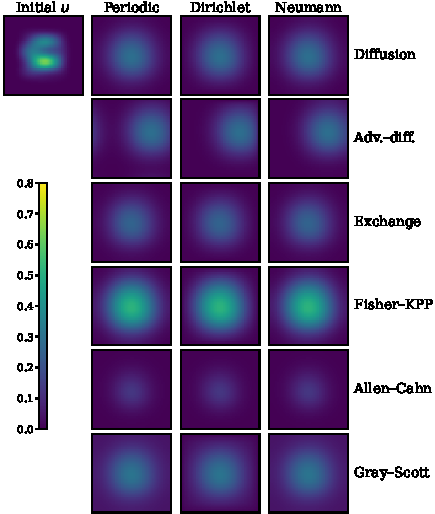
\includegraphics[width=0.94\columnwidth]{figures/fig_configurations.pdf}
\caption{The 18 problems that share one initial field (oscillation family, sample 1): $u$ at $t=1$ for six equations and three BCs, on a common color scale. Because the initial data vanish near the boundary and the horizon is short, the BC changes the solution much less than the equation does.}
\label{fig:configurations}
\end{figure}

\subsection{What We Ran and How We Score It}
All 5,400 trajectories, the reference distances, and the model-free baselines use all 100 samples. Running the three models on all 48,600 inputs was not possible on the two-core CPU we had (\cref{tab:model-inputs}). Before encoding any test input, we therefore fixed a smaller set: samples 0--9 of all 54 problems for the main runs (1,620 inputs per model), and samples 0--2 for the controls. Each model is always compared with the reference computed on the same samples. On these ten samples the reference rankings are almost identical to those from all 100 samples (mean Spearman correlation \refSubsetVsAll{}).

Within each IC family there are 153 pairs of distinct problems. Our main score is the Spearman rank correlation between the model similarity $S^{\mathrm{emb}}$ and $-D$ over these pairs, averaged over the three families. The second score is \emph{triplet accuracy}. Take an anchor problem and two others; if the reference says the first is closer to the anchor, does the model agree? Exact ties in the reference are skipped, and ties in the model count as one-half. We also split the pairs into those with the same BC and those with different BCs. The $54\times54$ matrix and the 100-frame reference are secondary.

Numerical error is far too small to affect these rankings. The error bound $\epsilon_i$ of \cref{prop:margin} is at most \refEpsLinear{} for the linear equations, where we compute it from exact solutions. For the nonlinear equations it is at most \refEpsNonlinear{}, estimated by refining the time step, with a safety factor of two. Reference distances range from \refDmin{} to \refDmax{}. All 7,344 triplets within IC families pass the test of \cref{prop:margin}, and the 10.3\% that involve only linear equations are proved up to rounding. Grid resolution matters just as little: on pilot samples, moving to a $128\times128$ grid changed the order of \pilotFlips{} of \pilotTriplets{} triplets (\cref{app:pilot}).

For uncertainty, we resample the ten samples with replacement (2,000 times), recompute both matrices, and report 95\% intervals. These intervals reflect the random ICs, not the choice of equations or BCs, and with ten samples they are rough. The pairs in a matrix are not independent, and nothing here supports claims about PDE families we did not test.

\subsection{Baselines and Controls}
\paragraph{Baselines.}
For text we use character 3--5-gram TF--IDF. For images we compare the raw pixels and, separately, the magnitudes of the low spatial Fourier modes ($|k|\le8$ in each direction). The physical cosine of \cref{sec:comparison} shows how well shape alone, without size, predicts the reference. The RMS distance on the numbers themselves is the reference, so it is not a baseline.

\paragraph{Initial frame only.}
An image showing only $t=0$ is the same for all 18 problems in an IC family. If a model is deterministic, all its similarities within a family equal one, the Spearman correlation is undefined, and triplet accuracy is $0.5$. This is the floor for a model that sees only the starting state.

\paragraph{Time order.}
We reverse the five snapshots in every image but leave the time labels in place. Reordering frames in the same way for every problem does not change the reference, so a model that responds to the fields themselves should give similar rankings.

\paragraph{Notation.}
We rewrite each description in an equivalent form: the Laplacian becomes second derivatives, diffusion moves to the end of each equation, and the coordinates $x,y$ become $\xi,\zeta$ in every formula. The rewritten problem is mathematically identical. Separately, four short heat-equation descriptions differ only in the diffusion coefficient of \cref{tab:calibration}.

\paragraph{Mismatched inputs.}
We pair the image of each problem with the description of the next equation in our list, keeping the same IC, BC, and sample. We then ask whether the joint similarities follow the reference for the image or the reference for the text.

\section{Results}
\label{sec:results}
\begin{table}[t]
\centering
\caption{Main result: Spearman correlation between model similarity $S^{\mathrm{emb}}$ and $-D$, averaged over the three IC families (153 pairs each). Samples 0--9, with the reference computed on the same samples. Brackets: 95\% bootstrap intervals. Baseline values in parentheses use all 100 samples.}
\label{tab:main}
\small
\setlength{\tabcolsep}{3.5pt}
\resizebox{\columnwidth}{!}{%
\begin{tabular}{lccc}
\toprule
Model & Text & Image & Joint \\
\midrule
EmbeddingGemma 2 & 0.21 {\scriptsize[0.21, 0.23]} & 0.76 {\scriptsize[0.73, 0.79]} & 0.23 {\scriptsize[0.22, 0.24]} \\
Qwen3-VL-Emb.-2B & 0.44 {\scriptsize[0.39, 0.45]} & 0.78 {\scriptsize[0.73, 0.83]} & 0.39 {\scriptsize[0.35, 0.40]} \\
GME-Qwen2-VL-2B & 0.46 {\scriptsize[0.44, 0.47]} & 0.83 {\scriptsize[0.75, 0.84]} & 0.50 {\scriptsize[0.47, 0.54]} \\
\midrule
Char.\ TF--IDF (text) & 0.35 {\scriptsize(0.36)} & -- & -- \\
Rendered pixels (image) & -- & 0.93 {\scriptsize(0.95)} & -- \\
Fourier magnitudes (image) & -- & 0.44 {\scriptsize(0.42)} & -- \\
Initial frame only (image) & -- & undefined & -- \\
\bottomrule
\end{tabular}}
\end{table}


\begin{figure*}[t]
\centering
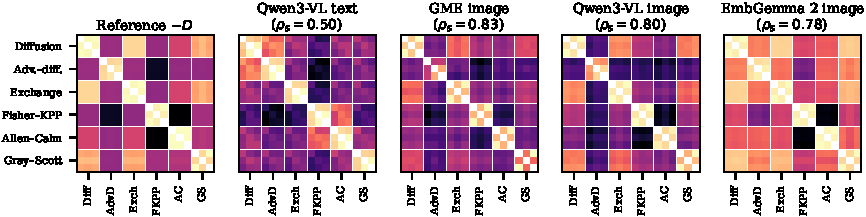
\includegraphics[width=\textwidth]{figures/fig_matrices.pdf}
\caption{Similarity between the 18 problems of the oscillation family (samples 0--9). Rows and columns are grouped by equation, with the periodic, Dirichlet, and Neumann versions inside each block. Brighter means more similar; the diagonal is left blank, and each panel has its own color scale. $\rho_s$ is the Spearman correlation with $-D$ for this family. Every model sees that the three BC versions of an equation are nearly the same. The image embeddings also recover much of the structure between equations; the text embedding recovers less of it.}
\label{fig:matrices}
\end{figure*}

\subsection{Main Results}
\paragraph{Images work best, but not better than pixels.}
With images, the three models reach Spearman correlations of \spImageMin--\spImageMax{} with the reference and triplet accuracies of \trImageMin--\trImageMax{} (\cref{tab:main,tab:secondary,fig:matrices}). That is real agreement. But every model falls short of simply comparing the pixels (\spPix{}), and lands close to the physical cosine (\spPhys{}), which ignores how strong a response is. For Qwen3-VL and GME, the image similarities actually follow the physical cosine more closely (Spearman \spQwImagePhys{} and \spGmeImagePhys{}) than they follow the reference. EmbeddingGemma 2 does not show this pattern (\spGemImagePhys{}). On this benchmark, the pretrained image features add nothing to the ranking that the pixels do not already contain, and they partly lose the size of the response.

\paragraph{Text descriptions agree only weakly.}
With text, the correlations are \spTextMin--\spTextMax{}. Qwen3-VL (\spQwText{}) and GME (\spGmeText{}) beat character TF--IDF (\spTfidf{}) by a small margin, and EmbeddingGemma 2 (\spGemText{}) does worse than it. All three models give the highest similarity to descriptions that share an equation (\cref{tab:factors}), which matches the reference. They do much worse at ordering different equations. On pairs with the same BC, where only the equation changes, the correlations are \spQwTextSame{}, \spGmeTextSame{}, and \spGemTextSame{}. In other words, the text embeddings recognize when two problems use the same equation, but they say little about how far apart the solutions of two different equations will end up.

\paragraph{Adding the image to the text helps little.}
With both inputs, the correlations are \spBothMin--\spBothMax{}. Each model stays close to its text-only score and far below its image-only score. Only GME improves noticeably over text alone (\spGmeBoth{} against \spGmeText{}). In every model, the description uses more tokens than the image (\cref{tab:model-inputs}). The mismatch control below shows that the models weigh the two inputs differently.

\paragraph{Other references.}
The image results hold up against the 100-frame reference (\spQwImageHund{}, \spGmeImageHund{}, and \spGemImageHund{} for Qwen3-VL, GME, and EmbeddingGemma 2) and across all 54 problems, where differences in the initial data also enter (\spQwImageFull{}, \spGmeImageFull{}, \spGemImageFull{}). Across all 54 problems, the text embeddings (\spQwTextFull{}, \spGmeTextFull{}, \spGemTextFull{}) fall far behind character TF--IDF (\spTfidfFull{}), which picks up the different IC formulas. Since every triplet is reliable, accuracy on reliable triplets equals overall accuracy, and triplets made only of linear equations show the same pattern (\cref{tab:secondary}).

\subsection{Controls}
\Cref{tab:controls} summarizes the controls. Encoding the same initial-frame image twice gave bit-identical embeddings in every model, so that control indeed has constant scores.

\paragraph{Time order.}
Reversing the snapshots hardly changes how well the image similarities match the reference (samples 0--2, original/reversed: \revOrigQw{}/\revRevQw{}, \revOrigGme{}/\revRevGme{}, and \revOrigGem{}/\revRevGem{} for Qwen3-VL, GME, and EmbeddingGemma 2). This is expected, since the reference does not depend on frame order. Yet the reversal moves each image embedding a long way. For Qwen3-VL and GME, an image and its reversed copy are about as similar (\revSelfQw{} and \revSelfGme{}) as the two least similar problems in an IC family (\rangeLoQwImage{} and \rangeLoGmeImage{}). For EmbeddingGemma 2 the value (\revSelfGem{}) lies inside that range. The models notice the layout, but nothing suggests that they use the direction of time.

\paragraph{Notation.}
Rewriting a description in equivalent notation changes its embedding a great deal. On average, an original description is more similar to its nearest \emph{different} problem (\notOtherQw{}, \notOtherGme{}, and \notOtherGem{} for Qwen3-VL, GME, and EmbeddingGemma 2) than to its own rewrite (\notSelfQw{}, \notSelfGme{}, and \notSelfGem{}). For GME and EmbeddingGemma 2 the effect is extreme: for \notAllGme{} and \notAllGem{} of descriptions, all 53 other problems, including those with different equations and different initial data, are closer to the original than its rewrite is. For Qwen3-VL, a median of \notCloserQw{} of the 53 are closer. Seen from the other side, a rewrite still finds its own original among the 54 descriptions of its sample in \notTopQw{}, \notTopGme{}, and \notTopGem{} of cases. The rewrite moves the embedding to a new region, not onto another problem. The rewritten descriptions match the reference no better than the originals (Spearman \notSpQw{}, \notSpGme{}, and \notSpGem{}, against \notSpOrigQw{}, \notSpOrigGme{}, and \notSpOrigGem{} on the same samples).

\paragraph{Mismatched inputs.}
When the image and the description disagree, Qwen3-VL follows the description: its joint similarities match the reference of the described problem (\misDeckQw{}) rather than the problem shown (\misImgQw{}). GME weighs the two about equally (\misDeckGme{} and \misImgGme{}), and EmbeddingGemma 2 leans toward the image (\misDeckGem{} and \misImgGem{}), even though its matched joint input does no better than text alone. So the image does reach the joint embedding, but in no model does it lift the joint score close to the image-only score.

\paragraph{Changing one coefficient.}
In the heat-equation test, where the four descriptions differ only in the diffusion coefficient, Qwen3-VL and EmbeddingGemma 2 rank the candidates in the correct order, $S(0.01,0.011)>S(0.01,0.02)>S(0.01,0.05)$. GME reverses it (similarities \heatValsGme{}).

\begin{table*}[t]
\centering
\caption{Further results on samples 0--9, averaged over IC families. Triplet accuracy for all triplets, for triplets whose order is guaranteed despite numerical error (``reliable''), and for triplets made only of linear equations, where the guarantee is exact. Spearman correlation for pairs with the same BC (45 per family) and with different BCs (108 per family), against the 100-frame reference, and over all 1,431 pairs of the 54 problems.}
\label{tab:secondary}
\small
\begin{tabular}{llccccccc}
\toprule
& & \multicolumn{3}{c}{Triplet accuracy} & \multicolumn{2}{c}{Spearman by BC} & \multicolumn{2}{c}{Spearman, other references} \\
\cmidrule(lr){3-5}\cmidrule(lr){6-7}\cmidrule(lr){8-9}
Model & Input & All & Reliable & Linear & Same BC & Diff.\ BC & 100 frames & All 54 \\
\midrule
EmbeddingGemma 2 & text & 0.57 & 0.57 & 0.70 & $-$0.26 & 0.32 & 0.24 & 0.28 \\
 & image & 0.78 & 0.78 & 0.79 & 0.64 & 0.80 & 0.70 & 0.83 \\
 & joint & 0.58 & 0.58 & 0.70 & $-$0.09 & 0.33 & 0.25 & 0.39 \\
Qwen3-VL-Emb.-2B & text & 0.65 & 0.65 & 0.66 & 0.22 & 0.53 & 0.36 & 0.20 \\
 & image & 0.79 & 0.79 & 0.83 & 0.69 & 0.82 & 0.88 & 0.77 \\
 & joint & 0.66 & 0.66 & 0.65 & 0.11 & 0.49 & 0.34 & 0.22 \\
GME-Qwen2-VL-2B & text & 0.64 & 0.64 & 0.69 & 0.18 & 0.55 & 0.49 & 0.29 \\
 & image & 0.84 & 0.84 & 0.87 & 0.74 & 0.86 & 0.87 & 0.74 \\
 & joint & 0.67 & 0.67 & 0.76 & 0.26 & 0.59 & 0.54 & 0.53 \\
TF--IDF & -- & 0.61 & 0.61 & 0.71 & 0.26 & 0.48 & -- & 0.67 \\
Pixels & -- & 0.95 & 0.95 & 0.96 & 0.90 & 0.94 & -- & 0.99 \\
Fourier & -- & 0.73 & 0.73 & 0.57 & 0.20 & 0.52 & -- & 0.40 \\
Phys.\ cosine & -- & 0.90 & 0.90 & 0.98 & 0.74 & 0.85 & -- & 0.64 \\
\bottomrule
\end{tabular}
\end{table*}

\begin{table*}[t]
\centering
\caption{Controls on samples 0--2 (heat test: four short descriptions). Time order: Spearman correlation with $-D$ for original/reversed images, and the average similarity between an image and its reversed copy. Notation: how often a rewritten description finds its own original among the 54 descriptions of its sample (top-1), and the average similarity of an original to its rewrite/to its most similar other problem. Mismatch: Spearman correlation of joint embeddings (image of one problem, description of the next equation) with the image's reference/the description's reference. Heat: whether $S(0.01,0.011)>S(0.01,0.02)>S(0.01,0.05)$ with text input.}
\label{tab:controls}
\small
\begin{tabular}{lcccccc}
\toprule
& \multicolumn{2}{c}{Time order (image)} & \multicolumn{2}{c}{Notation (text)} & Mismatch (joint) & Heat \\
\cmidrule(lr){2-3}\cmidrule(lr){4-5}
Model & Orig./rev. & Self-sim. & Top-1 & Rewrite/other & Image/text ref. & order \\
\midrule
EmbeddingGemma 2 & 0.75/0.81 & 0.999 & 0.38 & 0.973/0.998 & 0.41/0.19 & yes \\
Qwen3-VL-Emb.-2B & 0.70/0.74 & 0.988 & 0.77 & 0.956/0.995 & 0.09/0.36 & yes \\
GME-Qwen2-VL-2B & 0.77/0.74 & 0.985 & 0.50 & 0.958/0.997 & 0.41/0.40 & no \\
\bottomrule
\end{tabular}
\end{table*}


\section{Limitations}
The benchmark covers six small parabolic equations that share two fields. It leaves out turbulence, shocks, moving geometry, mixed physical units, and equations that need other kinds of boundary data. This keeps the comparisons easy to read and to reproduce, but it limits how far the results generalize. They describe agreement under this setup, not a universal ranking of PDEs.

The reference has a strong structure of its own. The initial fields vanish near the boundary and the time horizon is short, so changing the BC moves a solution much less than changing the equation (\cref{fig:configurations}). Rankings within an IC family are therefore mostly rankings of equations, and the split into same-BC and different-BC pairs should be read with this in mind. Other horizons, field scales, or IC distributions would change the rankings.

The embedding results use 10 of the 100 samples per problem, chosen in advance because only a two-core CPU was available. The reference rankings on these ten samples agree closely with those on all 100, but the bootstrap intervals rest on only ten samples. All three models ran in bfloat16 on a CPU. The checks in \cref{app:embedding-protocol,app:extra} suggest that this changes little, but a GPU run at each model's reference precision would be a useful replication.

Five snapshots are a compressed view of a solution. Measuring the reference on the same snapshots avoids giving the image models credit for information they never saw, and the 100-frame reference shows the cost of this compression. The image also fixes one way of drawing the data: a model can only see differences that survive the colormap, the $[0,0.8]$ range, and its own resizing.

Finally, the models were pretrained on large collections of text and images that may include PDEs. Their training data are not documented in enough detail to rule this out. New random ICs, controlled coefficients, and equivalent rewrites reduce the chance that a model has seen these exact problems, but they cannot prove that an equation was absent from pretraining.

\section{Conclusion}
We asked whether general-purpose multimodal embeddings rank PDE problems by how their solutions behave. To answer it, we simulated 5,400 trajectories with one validated solver, defined a reference distance whose rankings are reliable and partly proved, and queried three embedding models with descriptions, images, or both. On ten samples per problem, chosen in advance, image embeddings follow the reference moderately well (Spearman \spImageMin--\spImageMax{}) but do no better than raw pixels. Description embeddings follow it weakly (\spTextMin--\spTextMax{}), close to character $n$-grams, and for two of the models an equivalent rewrite moves a description further than any change of problem. Joint inputs stay close to the text. These models recognize solutions that \emph{look} alike much better than equations that \emph{behave} alike. Natural next steps are the full 100-sample run on a GPU, more coefficients and time horizons, and encoders trained with physical supervision, all evaluated under the same fixed protocol.

\FloatBarrier
\label{main-end}
\section*{Impact Statement}
This work tests whether embedding similarity reflects one specific, measurable kind of PDE behavior. Evidence of this kind can guide the use of embeddings for scientific search and organization. A high similarity score does not mean that two physical systems are interchangeable, or that either simulation is accurate. We release the problem definitions, numerical checks, and all results so that these limits stay visible.
\section*{AI Disclosure Statement}
ChatGPT helped with literature checks, drafting, derivations, and code for the earlier design draft. Claude (Anthropic) implemented the solver, the validation, the pilot, the main simulations, the embedding runs, and the analysis reported here, and revised the text. Every reported number comes from code that was actually run, and its outputs are included in the release; no result was estimated or filled in by a language model. The numerical checks are consistency checks, not formal proofs. The human authors must review the code, the paper, and the evidence before submission.
\bibliography{references}
\bibliographystyle{icml2027}
\clearpage
\appendix
\onecolumn
\section{Mathematical Details}
\label{app:simple-math}
All quantities below are defined on a fixed set of paired trajectories, fields, grid points, and observation times. They describe this experiment, not a universal ordering of PDEs.

\subsection{The Trajectory Distance}
\label{app:trajectory-distance}
Let $U_i^{(r)}(t_q)\in\mathbb R^{C\times n\times n}$ be sample $r$ of problem $i$ at time $t_q$, with $N=100$ samples, $C=2$ fields, and $n=64$. Choose positive time weights $w_q$ that sum to one. The five-frame distance uses $w_q=1/5$ and the 100-frame distance uses $w_q=1/100$. Define
\begin{equation}
 D_{i\ell}^2=\frac{1}{NCn^2}\sum_{r=1}^{N}\sum_{q=1}^{J}w_q
 \left\|U_i^{(r)}(t_q)-U_\ell^{(r)}(t_q)\right\|_F^2.
\label{eq:appendix-rms}
\end{equation}
Within an IC family, samples with the same index start from the same initial arrays. Across families, the pairing comes from the shared random seed.

\paragraph{Why this is a distance.}
Flatten one trajectory into
\[
 f_i^{(r)}=\left(\sqrt{\frac{w_q}{Cn^2}}\,
       \operatorname{vec}U_i^{(r)}(t_q)\right)_{q=1}^{J},
 \qquad F_i=\frac{1}{\sqrt N}\left(f_i^{(1)},\ldots,f_i^{(N)}\right).
\]
Then $D_{i\ell}=\|F_i-F_\ell\|_2$, so nonnegativity, symmetry, and the triangle inequality follow from the Euclidean norm. A zero distance means the recorded solutions are identical at every weighted time. $D$ is therefore a metric on distinct recorded solutions, but only a pseudometric on problems: two problems that agree on these samples need not agree for every initial condition.

\paragraph{Interpretation.}
Within an IC family, $D$ compares equations and BCs from shared initial data. Across families it also measures the change in initial data. A five-frame average is exactly that; we do not claim it equals a continuous-time integral.

\subsection{Dot Products and Normalization}
\label{app:physical-kernel}
The physical kernel $K_{i\ell}=F_i^\top F_\ell$ satisfies
\[
 D_{i\ell}^2=K_{ii}+K_{\ell\ell}-2K_{i\ell}.
\]
For the physical cosine, assume every flattened trajectory is nonzero and set $a_i^{(r)}=f_i^{(r)}/\|f_i^{(r)}\|_2$. Define
\[
 S_{i\ell}^{\mathrm{phys}}=\frac1N\sum_r a_i^{(r)\top}a_\ell^{(r)},
 \qquad A_i=\frac1{\sqrt N}(a_i^{(1)},\ldots,a_i^{(N)}).
\]
Then $S_{i\ell}^{\mathrm{phys}}=A_i^\top A_\ell$, $\|A_i\|_2=1$, and
\[
 \|A_i-A_\ell\|_2^2=2-2S_{i\ell}^{\mathrm{phys}}.
\]
The similarity matrix is positive semidefinite, because
$\sum_{i,\ell}c_i c_\ell S_{i\ell}^{\mathrm{phys}}=\|\sum_i c_i A_i\|_2^2\geq0$.
The same argument applies to the averaged embedding dot products of \cref{eq:embedding-score}. Normalizing each trajectory removes its size, so the physical cosine and the RMS distance are different targets and can rank pairs differently. A zero trajectory would have to be reported rather than divided by zero; none occurs here.

\subsection{When Numerical Error Can Change a Ranking}
\label{app:ranking-error}
Let $F_i$ be the exact solution and $\widetilde F_i$ its computed version, with $\|F_i-\widetilde F_i\|_2\leq\epsilon_i$. Write $\widetilde D_{i\ell}=\|\widetilde F_i-\widetilde F_\ell\|_2$. The reverse triangle inequality gives
\[
 |D_{i\ell}-\widetilde D_{i\ell}|
 \leq\|(F_i-\widetilde F_i)-(F_\ell-\widetilde F_\ell)\|_2
 \leq\epsilon_i+\epsilon_\ell.
\]
For an anchor $i$ and two candidates $\ell,k$, the condition
\[
 \widetilde D_{ik}-\widetilde D_{i\ell}
 >2\epsilon_i+\epsilon_\ell+\epsilon_k
\]
therefore guarantees $D_{i\ell}<D_{ik}$: the largest possible value of the first distance lies below the smallest possible value of the second. A difference between two step sizes or grids is useful evidence, but it is not automatically a rigorous bound. Here the exact target is the solution on the $64\times64$ grid, so only time-stepping and rounding errors enter $\epsilon_i$.

\subsection{Exact Solutions for the Linear Equations}
\label{app:linear-reference}
For diffusion and linear exchange, write
\[
 U_t=\mathbf D\Delta U+RU,\qquad
 \mathbf D=\operatorname{diag}(D_u,D_v),\qquad
 R=0\quad\text{or}\quad
 R=\kappa\begin{pmatrix}-1&1\\1&-1\end{pmatrix}.
\]
On the cell-centered grid with $h=1/n$, the one-dimensional Laplacian has off-diagonal entries $1/h^2$ and interior diagonal entries $-2/h^2$. Periodic boundaries wrap the neighbors. Zero Dirichlet ghost values are the negatives of the adjacent values, giving end diagonals $-3/h^2$. Zero Neumann ghost values copy the adjacent values, giving end diagonals $-1/h^2$.

The eigenvalues are
\[
\begin{array}{ll}
\text{Periodic:}&\lambda_k=-4h^{-2}\sin^2(\pi k/n),\quad k=0,\ldots,n-1,\\[2pt]
\text{Dirichlet:}&\lambda_k=-4h^{-2}\sin^2(\pi k/(2n)),\quad k=1,\ldots,n,\\[2pt]
\text{Neumann:}&\lambda_k=-4h^{-2}\sin^2(\pi k/(2n)),\quad k=0,\ldots,n-1.
\end{array}
\]
They follow by substituting the Fourier, cell-centered sine, and cell-centered cosine vectors into the stencils. In two dimensions the eigenvalues add, $\lambda_{k\ell}=\lambda_k+\lambda_\ell$. After transforming both fields to this basis, each two-component coefficient evolves as
\[
 \widehat U_{k\ell}(t)
 =e^{t(R+\lambda_{k\ell}\mathbf D)}\widehat U_{k\ell}(0).
\]
This gives the exact grid solution without any time stepping, and it does not require $R$ and $\mathbf D$ to commute. Different BCs use different eigenvectors, so fields are transformed back to the grid before they are compared. Advection--diffusion separates into an $x$ part and a $y$ part, so its exact grid solution is $e^{tA_x}U_0e^{tA_y^\top}$ for each field, where $A_x$ and $A_y$ are the one-dimensional operators.

\paragraph{Continuous test solutions.}
On the unit interval, the continuous Laplacian has eigenvalues $-4\pi^2k^2$ for periodic modes, and $-\pi^2k^2$ for Dirichlet ($k\geq1$) and Neumann ($k\geq0$) modes; in two dimensions they add. If $\phi$ is such an eigenfunction with eigenvalue $\lambda$, the initial field $U_0(x,y)=\phi(x,y)b$ has the exact solution
\[
 U(t,x,y)=\phi(x,y)e^{t(R+\lambda\mathbf D)}b.
\]
We use these solutions only to test the solver against the continuous PDE; they are not benchmark initial conditions.

\section{Solver Checks, Pilot, and Fixed Protocol}
\label{app:validation}
\subsection{Solver Checks}
All checks used pilot samples (index 100 or higher) or constructed test fields. No test sample was simulated before the protocol was fixed. The transform-based Laplacians match the five-point stencils to a relative error below $5\times10^{-16}$ for all three BCs, and the centered differences match the corresponding matrices exactly. We also checked the exact linear solutions themselves against full $2n^2\times2n^2$ matrix exponentials on an $8\times8$ grid; they agree to $3.4\times10^{-15}$.

\Cref{tab:validation} summarizes the rest. Diffusion is solved exactly in the transform basis, so its only error is rounding. For advection--diffusion and linear exchange, the error against the exact grid solution falls by a factor of about 16 each time the step is halved, as expected for a fourth-order method. The continuous test solutions for diffusion and exchange show spatial convergence orders between \valOrderMin{} and \valOrderMax{} for every BC. For every equation, the difference from the $256\times256$ solution is 5.0 times larger at $64\times64$ than at $128\times128$, which is the ratio expected for second-order convergence.

\begin{table}[h]
\centering
\caption{Solver checks on pilot samples. Time error: largest absolute error with four steps per output interval, measured against the exact grid solution (linear equations) or against a run with four times as many steps (nonlinear equations). Space: largest five-frame RMS difference from the $256\times256$ solution after averaging to the coarser grid. Exponax: largest five-frame RMS difference from an independent spectral solver at $64\times64$ (periodic BC only).}
\label{tab:validation}
\small
\begin{tabular}{lcccc}
\toprule
Equation & Time error & Space, $64^2$ & Space, $128^2$ & Exponax, $64^2$ \\
\midrule
Diffusion & $2.9\times10^{-14}$ (exact) & $1.0\times10^{-4}$ & $2.0\times10^{-5}$ & $5.0\times10^{-5}$ \\
Advection--diffusion & $2.3\times10^{-10}$ (exact) & $4.0\times10^{-4}$ & $8.0\times10^{-5}$ & $2.4\times10^{-4}$ \\
Linear exchange & $9.2\times10^{-13}$ (exact) & $9.1\times10^{-5}$ & $1.8\times10^{-5}$ & -- \\
Fisher--KPP & $2.7\times10^{-12}$ (refined) & $1.2\times10^{-4}$ & $2.4\times10^{-5}$ & $6.5\times10^{-5}$ \\
Allen--Cahn (shifted) & $4.9\times10^{-12}$ (refined) & $9.7\times10^{-5}$ & $1.9\times10^{-5}$ & $5.0\times10^{-5}$ \\
Gray--Scott & $1.1\times10^{-12}$ (refined) & $1.0\times10^{-4}$ & $2.1\times10^{-5}$ & $4.8\times10^{-5}$ \\
\bottomrule
\end{tabular}
\end{table}


\paragraph{Independent periodic check.}
For periodic BCs we ran Exponax \citep{exponax_docs} (version 0.2.1, float64) on diffusion, advection--diffusion, Fisher--KPP, Allen--Cahn, and Gray--Scott, from the same pilot fields. For Allen--Cahn we used the substitution $w=2u-1$, which turns our shifted cubic into $w_t=\nu\Delta w+\tfrac a4(w-w^3)$. Exponax is a spectral method and is very accurate in space for these smooth fields, so the difference between the two solvers measures our finite-difference error. Refining from $n=64$ to $n=128$ shrinks this difference by a median factor of \expoRatio{}, consistent with second order, and the largest difference at $64\times64$ is \expoMax{}. Exponax has no linear-exchange solver; for that equation the exact grid solution serves instead.

\subsection{Pilot}
\label{app:pilot}
The pilot (\texttt{scripts/pilot.py}, samples 100--119) evaluated the criteria listed in \cref{sec:benchmark}. All passed, and the coefficients were not changed. The largest values at the five observed times were \pilotMaxU{} for $u$ and \pilotMaxV{} for $v$, which set the image color range to $[0,0.8]$ for both fields. On samples 100--104, the distance matrices computed on the $64\times64$ and $128\times128$ grids had Spearman correlations of at least \pilotSpearmanMin{}, and only \pilotFlips{} of \pilotTriplets{} triplets changed order. Grid resolution therefore has almost no effect on the reference rankings.

\subsection{Fixed Protocol and Run Record}
After the pilot, and before any test sample was simulated or encoded, we wrote \texttt{benchmark/frozen\_protocol.json}. It fixes the coefficients, solver settings, image rendering, model versions and input formats, the ten-sample subset, the controls, the error test, the baselines, and the definitions of all scores. It also stores SHA-256 hashes of the scripts that existed at that point. The analysis, table, and figure scripts were written afterwards but before any embedding output was looked at, and they follow the fixed definitions. The Exponax check and the recorded check of the exact linear solutions were also added later; they use only pilot or synthetic data. A \texttt{--float32} option for the planned precision check was added to the embedding script without changing its default behavior.

The main simulation took \simSeconds{} minutes on two CPU cores. No trajectory failed, and no value was clipped or changed. Stored values lie in $[\simMin,\ \simMax]$. The \simOOR{} image pixels outside the color range are all tiny negative rounding errors, which the colormap shows as zero. The run record stores a SHA-256 hash of every stored array and of every full 100-frame trajectory. The full trajectories (17.7\,GB) are not kept, but they can be regenerated exactly and checked against these hashes.

\section{Reproducibility Details}
\label{app:reproducibility}
\subsection{Initial Conditions}
\texttt{scripts/make\_decks.py} defines the IC distributions. For each sample index $r\in\{0,\ldots,99\}$ it draws a fixed two-channel random array with NumPy's PCG64 generator and seed sequence $[20261118,r]$. Each IC family maps the same random array to its own parameters, and the two fields use separate rows. Parameters are rounded to eight decimal places before the field is evaluated, so the saved numbers define the actual initial field.

Let $\alpha\sim\mathcal U[0.2,0.8]$, $m_x,m_y\sim\mathcal U[0.25,0.75]$, and $\sigma\sim\mathcal U[0.08,0.18]$, and define
\[
 B(x,y;m_x,m_y,\sigma)=
 \exp\!\left[-\frac{(x-m_x)^2+(y-m_y)^2}{2\sigma^2}\right].
\]
Each field uses one of the following:
\begin{align*}
 \text{Single bump:}\quad &\alpha w(x,y)B(x,y;m_x,m_y,\sigma),\\
 \text{Oscillations:}\quad &\frac{\alpha w(x,y)}{1.5}
 \big[1+0.5\cos(2\pi k_xx+\phi_x)\cos(2\pi k_yy+\phi_y)\big],\\
 \text{Three patches:}\quad &\alpha w(x,y)
 \frac{\sum_{\ell=1}^3 b_\ell B(x,y;m_{x,\ell},m_{y,\ell},\sigma_\ell)}
 {\sum_{\ell=1}^3 b_\ell}.
\end{align*}
Here $k_x,k_y$ are uniform on $\{1,2,3\}$, the phases are uniform on $[0,2\pi)$, and the patch weights $b_\ell$ are uniform on $[0.2,1]$. Patch centers and widths use the single-bump ranges. Every initial field lies in $[0,0.8]$. The same parameter bank is used for all equations and BCs. Linking different IC families through a shared seed is a design choice; it is not an optimal coupling between their distributions.

\subsection{Descriptions and Records}
The release contains 54 JSON problem files, the 300-sample IC parameter bank, and all 5,400 text and JSON descriptions. Running the generator with \texttt{--all-realizations} rebuilds the full set; without it, the generator writes three examples.

The text given to a model contains the two equations with all coefficients, the two explicit initial fields, the boundary data, the domain, and the time interval. The JSON version adds the IC family, sample index, grid, saved times, and observed frames. Solver settings, checksums, and diagnostics are stored in \texttt{benchmark/results/simulation\_manifest.json}. Model versions, preprocessing settings, token counts, and timings are stored next to the embeddings. Keeping these records out of the model text means that no solver setting or label can leak into a model input.

Below is the complete text given to a model for one sample of advection--diffusion with a single-bump IC and zero Neumann BC (long lines are wrapped for display). Its equivalent form would be $u_t=0.01(u_{xx}+u_{yy})-0.25u_x-0.10u_y$, and likewise for $v$. A model never has to guess what a named solver's defaults would be.
\begin{lstlisting}[basicstyle=\ttfamily\scriptsize,breaklines=true,columns=fullflexible,frame=single]
Equation:
\partial_t u=D_u\Delta u-c_x\partial_xu-c_y\partial_yu,\qquad \partial_t v=D_v\Delta v-c_x\partial_xv-c_y\partial_yv.

Parameters:
D_u=0.01000000,\quad D_v=0.00500000,\quad c_x=0.25000000,\quad c_y=0.10000000.

Initial condition:
\eta(s)=\begin{cases}\exp\!\left(4-\frac{1}{s(1-s)}\right),&0<s<1,\\0,&s\in\{0,1\}.\end{cases}
u(0,x,y)=0.41581429\,\eta(x)\eta(y)\,\exp\!\left[-\frac{(x-0.52007856)^2+(y-0.44353150)^2}{2(0.08503441)^2}\right].
v(0,x,y)=0.62013414\,\eta(x)\eta(y)\,\exp\!\left[-\frac{(x-0.74287585)^2+(y-0.27895931)^2}{2(0.13975413)^2}\right].

Boundary:
\partial_{\mathbf n}U(t,x,y)=0\quad\text{for }(x,y)\in\partial\Omega.

Domain:
\Omega=[0,1]^2,\qquad U=(u,v)^\top,\qquad \Delta=\partial_{xx}+\partial_{yy}.\quad x_p=(p+\tfrac12)/64,\ y_q=(q+\tfrac12)/64,\ p,q=0,\ldots,63.

Time:
0\leq t\leq1,\qquad t_n=n/99,\quad n=0,\ldots,99.\quad \text{Observed frames: }n\in\{0,25,50,74,99\}.
\end{lstlisting}

\subsection{Solver Settings}
Cell centers are $x_p=(p+1/2)/64$ and $y_q=(q+1/2)/64$ for $p,q=0,\ldots,63$, and arrays are ordered (field, $x$, $y$). The exact linear solutions in \cref{app:linear-reference} use the same stencil and ghost values as the solver, so they test the same grid equations. One solver serves all six equations, so no equation is tied to a different grid or boundary treatment.

Output times and solver steps differ even for diffusion. With $h=1/64$ and $\nu_{\max}=0.01$, an explicit five-point scheme would need $\delta t\le h^2/(4\nu_{\max})\approx0.00610$, while outputs are $1/99\approx0.01010$ apart. ETDRK4 handles diffusion exactly and uses $\delta t=1/396$ for the remaining terms. No trajectory failed, was dropped, or was clipped; stored values lie in $[\simMin,\ \simMax]$.

APEBench's periodic interface uses \texttt{num\_train\_samples=100} and \texttt{train\_temporal\_horizon=99} for 100 samples with 100 saved states \citep{apebench_base_docs}. Its default time steps and IC generators differ from ours, so the periodic check in \cref{app:validation} calls the Exponax solvers directly with our initial arrays.

\subsection{Embedding Protocol}
\label{app:embedding-protocol}
The model versions are \texttt{google/embeddinggemma-2} (revision \texttt{f9972ac}), \texttt{Qwen/Qwen3-VL-Embedding-2B} (\texttt{9f2f7e7}), and \texttt{Alibaba-NLP/gme-Qwen2-VL-2B-Instruct} (\texttt{9cfa641}); the full hashes are in the protocol file. Their model cards describe combined text and image inputs \citep{embeddinggemma2_modelcard,qwen3vl_embedding_modelcard,gme_modelcard}, and the Qwen3-VL and GME reports describe their training and evaluation \citep{li2026qwen3vl,zhang2024gme}.

Each model gets its documented input format, with one fixed prompt for every input. EmbeddingGemma 2 receives the symmetric prefix ``\texttt{task: sentence similarity | query: }'' on inputs with text, no prefix on images, and, for joint inputs, the description followed by the \texttt{<|image|>} placeholder; we use the checkpoint's mean pooling. Qwen3-VL-Embedding follows its official script: the instruction ``Represent the user's input.'', image before text, the generation prompt, last-token pooling, and image resizing by \texttt{qwen-vl-utils}. GME follows its reference code \texttt{gme\_inference.py}: the system prompt ``You are a helpful assistant.'', image before text, a final \texttt{<|endoftext|>} token, sequential positions, 256--1280 image tokens, and a limit of 1,800 tokens. We do not use separate query and document prompts, because our score in \cref{eq:embedding-score} treats both sides of a pair the same way. All models run in bfloat16 with batch size one, which this CPU supports natively, and every output is renormalized in float32 at full size. No input was truncated (\cref{tab:model-inputs}).

Before encoding any test input, we checked each interface on a pilot image; the results are stored in \texttt{benchmark/embedding\_interface\_checks.json}. Our GME code produces the same tokens and image grid as the official code run under transformers 4.51.3, and the embeddings agree to a cosine similarity of at least 0.997; the remaining difference comes from bfloat16 arithmetic in different library versions. Our Qwen3-VL code agrees with the sentence-transformers interface on the model card (cosine at least 0.998). Putting the text before the image instead changes the Qwen3-VL joint embedding a lot (cosine 0.905 with the official order), so input order is part of the protocol.

\subsection{What Was Encoded}
On a CPU with two cores and no GPU, encoding all $3\times3\times5400=48{,}600$ main inputs was not possible. The protocol therefore fixed a smaller set in advance: samples 0--9 of all 54 problems with all three input types (1,620 inputs per model), and samples 0--2 for the controls (162 reversed images, 162 rewritten descriptions, 162 mismatched pairs, 18 initial-frame images, and four heat-equation descriptions per model). Every model and baseline is compared with the reference computed on the same samples. The full run only needs \texttt{scripts/run\_embeddings.py --realizations 100}.

\subsection{Statistics and Release}
Samples with index 100 or higher were used only for setup and image scaling; the test set is samples 0--99. Bootstrap intervals resample the encoded samples (2,000 times) and are rough with ten samples. Every encoding attempt is logged; a failure would appear in the embedding records, and none occurred.

The release contains the problem files, the parameter bank, all descriptions, the solver and its checks, the pilot and run records, the per-sample reference terms, all embeddings, the analysis code, and the generated tables. It also includes the 540 images that were encoded in the main runs (samples 0--9). The five-frame arrays (0.9\,GB) and the remaining images are regenerated by \texttt{scripts/run\_simulations.py} and checked against the recorded hashes.

\section{Additional Results}
\label{app:extra}
\begin{figure}[h]
\centering
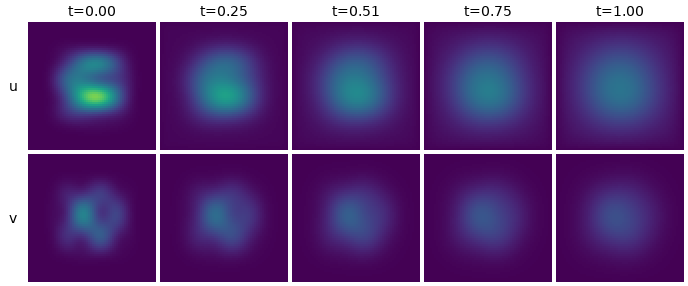
\includegraphics[width=0.62\textwidth]{figures/example_sheet.png}
\caption{A real image input: Gray--Scott, oscillation IC, zero Dirichlet BC, sample 1. Rows are the fields $u$ and $v$; columns are the five observed times. Every image uses this layout, colormap, and color range.}
\label{fig:example-sheet}
\end{figure}

\begin{table}[h]
\centering
\caption{Spearman correlation with $-D$ for each IC family (samples 0--9), and the range of similarities between different problems in the same family.}
\label{tab:perfamily}
\small
\begin{tabular}{llcccc}
\toprule
Model & Input & Bump & Oscill. & Patches & $S^{\mathrm{emb}}$ range \\
\midrule
EmbeddingGemma 2 & text & 0.24 & 0.17 & 0.24 & 0.985--0.999 \\
 & image & 0.72 & 0.78 & 0.77 & 0.997--1.000 \\
 & joint & 0.24 & 0.16 & 0.28 & 0.980--0.999 \\
Qwen3-VL-Emb.-2B & text & 0.37 & 0.50 & 0.44 & 0.898--0.996 \\
 & image & 0.83 & 0.80 & 0.72 & 0.987--0.999 \\
 & joint & 0.34 & 0.44 & 0.39 & 0.882--0.997 \\
GME-Qwen2-VL-2B & text & 0.47 & 0.42 & 0.48 & 0.973--0.998 \\
 & image & 0.87 & 0.83 & 0.81 & 0.985--0.999 \\
 & joint & 0.58 & 0.50 & 0.42 & 0.972--0.998 \\
\bottomrule
\end{tabular}
\end{table}

\begin{table}[h]
\centering
\caption{Exploratory (not planned in advance): average similarity between problems in the same IC family, grouped by what they share: the same equation with a different BC (9 pairs per family), the same BC with a different equation (45), or neither (99). The last row gives the average reference distance for the same groups (smaller means more similar).}
\label{tab:factors}
\small
\begin{tabular}{llccc}
\toprule
Model & Input & Same eq. & Same BC & Neither \\
\midrule
EmbeddingGemma 2 & text & 0.9971 & 0.9920 & 0.9896 \\
 & image & 0.9999 & 0.9989 & 0.9989 \\
 & joint & 0.9960 & 0.9930 & 0.9902 \\
Qwen3-VL-Emb.-2B & text & 0.9906 & 0.9513 & 0.9434 \\
 & image & 0.9983 & 0.9920 & 0.9920 \\
 & joint & 0.9923 & 0.9408 & 0.9368 \\
GME-Qwen2-VL-2B & text & 0.9968 & 0.9838 & 0.9812 \\
 & image & 0.9969 & 0.9899 & 0.9898 \\
 & joint & 0.9953 & 0.9835 & 0.9803 \\
\midrule
Reference $D$ & -- & 0.0019 & 0.0343 & 0.0343 \\
\bottomrule
\end{tabular}
\end{table}


\paragraph{Precision.}
As planned in the protocol, we re-encoded sample 0 of all 54 problems with EmbeddingGemma 2 in float32. The lowest cosine similarity between the float32 and bfloat16 embeddings of the same input is \precTextMinCos{} for text, \precImageMinCos{} for images, and \precBothMinCos{} for joint inputs. The two precisions rank pairs almost identically (mean Spearman correlation \precTextSS{}, \precImageSS{}, and \precBothSS{}). Agreement with the reference on this sample changes from \precTextRefB{} to \precTextRefA{} (text), from \precImageRefB{} to \precImageRefA{} (image), and from \precBothRefB{} to \precBothRefA{} (joint) when we switch from bfloat16 to float32. Reduced precision does not explain the results.

\end{document}
